\documentclass[a4paper,titlepage,11pt,twosides,floatssmall]{mwrep}
\usepackage[left=2.5cm,right=2.5cm,top=2.5cm,bottom=2.5cm]{geometry}
\usepackage[OT1]{fontenc}
\usepackage{polski}
\usepackage{amsmath}
\usepackage{amsfonts}
\usepackage{amssymb}
\usepackage{graphicx}
\usepackage{url}
\usepackage{tikz}
\usepackage{float}
\usetikzlibrary{arrows,calc,decorations.markings,math,arrows.meta}
\usepackage{rotating}
\usepackage[percent]{overpic}
\usepackage[utf8]{inputenc}
\usepackage{xcolor}
\usepackage{pgfplots}
\usetikzlibrary{pgfplots.groupplots}
\usepackage{listings}
\usepackage{matlab-prettifier}
\usepackage{siunitx}
\usepackage{placeins}
\definecolor{szary}{rgb}{0.95,0.95,0.95}
\sisetup{detect-weight,exponent-product=\cdot,output-decimal-marker={,},per-mode=symbol,binary-units=true,range-phrase={-},range-units=single}

%konfiguracje pakietu listings
\lstset{
	backgroundcolor=\color{szary},
	frame=single,
	breaklines=true,
}
\lstdefinestyle{customlatex}{
	basicstyle=\footnotesize\ttfamily,
	%basicstyle=\small\ttfamily,
}
\lstdefinestyle{customc}{
	breaklines=true,
	frame=tb,
	language=C,
	xleftmargin=0pt,
	showstringspaces=false,
	basicstyle=\small\ttfamily,
	keywordstyle=\bfseries\color{green!40!black},
	commentstyle=\itshape\color{purple!40!black},
	identifierstyle=\color{blue},
	stringstyle=\color{orange},
}
\lstdefinestyle{custommatlab}{
	captionpos=t,
	breaklines=true,
	frame=tb,
	xleftmargin=0pt,
	language=matlab,
	showstringspaces=false,
	%basicstyle=\footnotesize\ttfamily,
	basicstyle=\scriptsize\ttfamily,
	keywordstyle=\bfseries\color{green!40!black},
	commentstyle=\itshape\color{purple!40!black},
	identifierstyle=\color{blue},
	stringstyle=\color{orange},
}

%wymiar tekstu (bez żywej paginy)
\textwidth 160mm \textheight 247mm

%ustawienia pakietu pgfplots
\pgfplotsset{
tick label style={font=\scriptsize},
label style={font=\small},
legend style={font=\small},
title style={font=\small}
}

\def\figurename{Rys.}
\def\tablename{Tab.}

%konfiguracja liczby pływających elementów
\setcounter{topnumber}{0}%2
\setcounter{bottomnumber}{3}%1
\setcounter{totalnumber}{5}%3
\renewcommand{\textfraction}{0.01}%0.2
\renewcommand{\topfraction}{0.95}%0.7
\renewcommand{\bottomfraction}{0.95}%0.3
\renewcommand{\floatpagefraction}{0.35}%0.5

\begin{document}
\frenchspacing
\pagestyle{uheadings}

%strona tytułowa
\title{\bf Sprawozdanie z projektu nr 5, zadanie nr 6\vskip 0.1cm}
\author{Mateusz Koroś, Ksawery Pasikowski, Mateusz Morusiewicz}
\date{2017}

\makeatletter
\renewcommand{\maketitle}{\begin{titlepage}
\begin{center}{\LARGE {\bf
Wydział Elektroniki i Technik Informacyjnych}}\\
\vspace{0.4cm}
{\LARGE {\bf Politechnika Warszawska}}\\
\vspace{0.3cm}
\end{center}
\vspace{5cm}
\begin{center}
{\bf \LARGE Projektowanie układów sterowania\\ (projekt grupowy) \vskip 0.1cm}
\end{center}
\vspace{1cm}
\begin{center}
{\bf \LARGE \@title}
\end{center}
\vspace{2cm}
\begin{center}
{\bf \Large \@author \par}
\end{center}
\vspace*{\stretch{6}}
\begin{center}
\bf{\large{Warszawa, \@date\vskip 0.1cm}}
\end{center}
\end{titlepage}
}
\makeatother

\maketitle
\tableofcontents
\chapter*{Zad. 1}
Poprawność punktu pracy została udowodniona poprzez sprawdzenie, czy obiekt, będący w punkcie pracy, pozostanie w nim, jeśli wartości sterowania pozostaną takie same. Zostało to wykonane za pomocą komendy:
\begin{lstlisting}[style=Matlab-editor]
[y1_ust, y2_ust, y3_ust] = symulacja_obiektu6(0, 0, 0, 0, 0, 0, ...
0, 0, 0, 0, 0, 0, 0, 0, 0, 0, 0, 0, 0, 0, 0, 0, 0, 0, 0, 0, 0, 0)
\end{lstlisting}
Co dało wynik $ [0, 0, 0] $, co dowodzi, że punktem pracy rzeczywiście jest punkt $u_{1}=u_{2}=u_{3}=u_{4}=y_{1}=y_{2}=y_{3}=0$

\chapter*{Zad. 2}
Wszystkie sterowania zostały wzbudzone z wartości $ 0 $ do $ 1 $. W momencie skoku jednego sterowania wszystkie inne były wyłączone. Odpowiedzi skokowe widać na rysunkach.

\begin{figure}[]
	\centering
	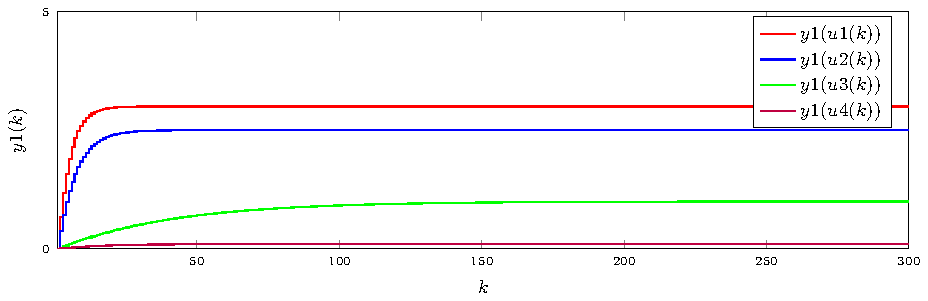
\includegraphics[scale=1]{../wykresy/zad2_y1.pdf}
	\caption{Odpowiedzi torów $y1(u1)$, $y1(u2)$, $y1(u3)$ i $y1(u4)$}
	\label{zad2_odpskok1}
\end{figure}


\begin{figure}[]
	\centering
	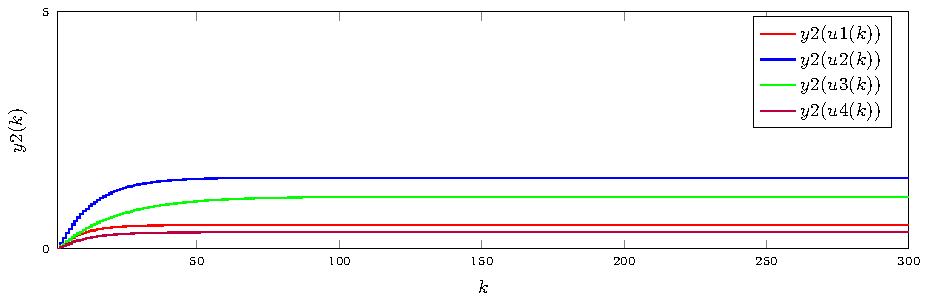
\includegraphics[scale=1]{../wykresy/zad2_y2.pdf}
	\caption{Odpowiedzi torów $y2(u1)$, $y2(u2)$, $y2(u3)$ i $y2(u4)$}
	\label{zad2_odpskok2}
\end{figure}

\begin{figure}[]
	\centering
	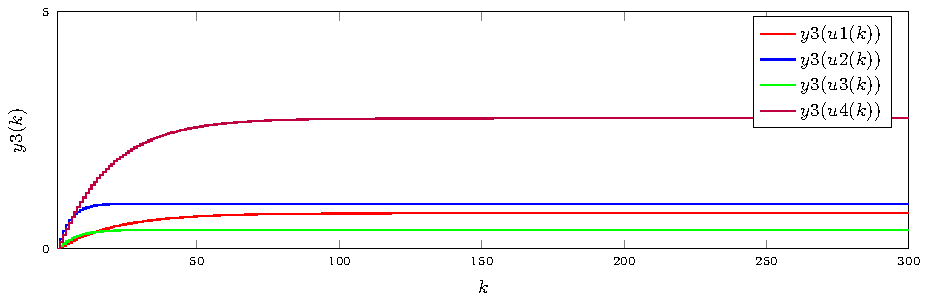
\includegraphics[scale=1]{../wykresy/zad2_y3.pdf}
	\caption{Odpowiedzi torów $y3(u1)$, $y3(u2)$, $y3(u3)$ i $y3(u4)$}
	\label{zad2_odpskok3}
\end{figure}



\chapter*{Zad. 3}
\section*{PID}
\begin{lstlisting}[style=Matlab-editor]
function [ y, u, E, yzad ] = policzPID( Kp1_, Ti1_, Td1_, Kp2_, ...
Ti2_, Td2_, Kp3_, Ti3_, Td3_, Kk_, option)
Kp1 = Kp1_;
Ti1 = Ti1_;
Td1 = Td1_;
Kp2 = Kp2_;
Ti2 = Ti2_;
Td2 = Td2_;
Kp3 = Kp3_;
Ti3 = Ti3_;
Td3 = Td3_;

Kk = Kk_;
Tp = 0.5;

r2_1 = (Kp1 * Td1) / Tp ;
r1_1 = Kp1 * ( (Tp/(2*Ti1)) - 2*(Td1/Tp) - 1 ) ;
r0_1 = Kp1 * ( 1 + Tp/(2*Ti1) + Td1/Tp ) ;

r2_2 = (Kp2 * Td2) / Tp ;
r1_2 = Kp2 * ( (Tp/(2*Ti2)) - 2*(Td2/Tp) - 1 ) ;
r0_2 = Kp2 * ( 1 + Tp/(2*Ti2) + Td2/Tp ) ;

r2_3 = (Kp3 * Td3) / Tp ;
r1_3 = Kp3 * ( (Tp/(2*Ti3)) - 2*(Td3/Tp) - 1 ) ;
r0_3 = Kp3 * ( 1 + Tp/(2*Ti3) + Td3/Tp ) ;

% warunki poczatkowe

u1(1:11) = 0 ;
y1(1:11) = 0 ;
e1(1:11) = 0 ;
u2(1:11) = 0 ;
y2(1:11) = 0 ;
e2(1:11) = 0 ;
u4(1:11) = 0 ;
y3(1:11) = 0 ;
e3(1:11) = 0 ;

u3(1:Kk) = 0 ; % ma najmniejsze wzmocnienie



index1 = 1;
index2 = 1;
index3 = 1;


yzads1 = [0.9 -0.1 0.3 1];
yzads2 = [-0.5 0 0.2 -0.3];   
yzads3 = [0.3 -0.2 0.1 0.6]; 

yzad1 = yzads1(index1);
yzad2 = yzads2(index2);
yzad3 = yzads3(index3);
yzadVec1(1:Kk) = yzad1;
yzadVec2(1:Kk) = yzad2;
yzadVec3(1:Kk) = yzad3;

% glowna petla symulacji
for k = 12 : Kk
if mod(k,200) == 0
index1 = index1 + 1;
if index1 > length(yzads1)
index1 = length(yzads1);
end
yzad1 = yzads1(index1);
end
yzadVec1(k) = yzad1;

if mod(k,130) == 0
index2 = index2 + 1;
if index2 > length(yzads2)
index2 = length(yzads2);
end
yzad2 = yzads2(index2);
end
yzadVec2(k) = yzad2;

if mod(k,220) == 0
index3 = index3 + 1;
if index3 > length(yzads3)
index3 = length(yzads3);
end
yzad3 = yzads3(index3);
end
yzadVec3(k) = yzad3;

[y1(k), y2(k), y3(k)] = symulacja_obiektu6( ...
u1(k-1), u1(k-2), u1(k-3), u1(k-4), ...
u2(k-1), u2(k-2), u2(k-3), u2(k-4), ...
u3(k-1), u3(k-2), u3(k-3), u3(k-4), ...
u4(k-1), u4(k-2), u4(k-3), u4(k-4), ...
y1(k-1), y1(k-2), y1(k-3), y1(k-4), ...
y2(k-1), y2(k-2), y2(k-3), y2(k-4), ...
y3(k-1), y3(k-2), y3(k-3), y3(k-4));


e1(k) = yzad1 - y1(k) ;
e2(k) = yzad2 - y2(k) ;
e3(k) = yzad3 - y3(k) ;

if option == 1
u1(k) = r2_1 * e1(k-2) + r1_1 * e1(k-1) + r0_1 * e1(k) + u1(k-1) ;
u2(k) = r2_2 * e2(k-2) + r1_2 * e2(k-1) + r0_2 * e2(k) + u2(k-1) ;
u4(k) = r2_3 * e3(k-2) + r1_3 * e3(k-1) + r0_3 * e3(k) + u4(k-1) ;
elseif option == 2
u1(k) = r2_1 * e1(k-2) + r1_1 * e1(k-1) + r0_1 * e1(k) + u1(k-1) ;
u2(k) = r2_2 * e3(k-2) + r1_2 * e3(k-1) + r0_2 * e3(k) + u2(k-1) ;
u4(k) = r2_3 * e2(k-2) + r1_3 * e2(k-1) + r0_3 * e2(k) + u4(k-1) ;
elseif option == 3
u1(k) = r2_1 * e2(k-2) + r1_1 * e2(k-1) + r0_1 * e2(k) + u1(k-1) ;
u2(k) = r2_2 * e1(k-2) + r1_2 * e1(k-1) + r0_2 * e1(k) + u2(k-1) ;
u4(k) = r2_3 * e3(k-2) + r1_3 * e3(k-1) + r0_3 * e3(k) + u4(k-1) ;
elseif option == 4
u1(k) = r2_1 * e2(k-2) + r1_1 * e2(k-1) + r0_1 * e2(k) + u1(k-1) ;
u2(k) = r2_2 * e3(k-2) + r1_2 * e3(k-1) + r0_2 * e3(k) + u2(k-1) ;
u4(k) = r2_3 * e1(k-2) + r1_3 * e1(k-1) + r0_3 * e1(k) + u4(k-1) ;
elseif option == 5
u1(k) = r2_1 * e3(k-2) + r1_1 * e3(k-1) + r0_1 * e3(k) + u1(k-1) ;
u2(k) = r2_2 * e1(k-2) + r1_2 * e1(k-1) + r0_2 * e1(k) + u2(k-1) ;
u4(k) = r2_3 * e2(k-2) + r1_3 * e2(k-1) + r0_3 * e2(k) + u4(k-1) ;
elseif option == 6
u1(k) = r2_1 * e3(k-2) + r1_1 * e3(k-1) + r0_1 * e3(k) + u1(k-1) ;
u2(k) = r2_2 * e2(k-2) + r1_2 * e2(k-1) + r0_2 * e2(k) + u2(k-1) ;
u4(k) = r2_3 * e1(k-2) + r1_3 * e1(k-1) + r0_3 * e1(k) + u4(k-1) ;
end

end

E1 = (yzadVec1 - y1) * (yzadVec1 - y1)';
E2 = (yzadVec2 - y2) * (yzadVec2 - y2)';
E3 = (yzadVec3 - y3) * (yzadVec3 - y3)';
E = E1 + E2 + E3;

yzad = zeros(3, Kk);
yzad(1, :) = yzadVec1;
yzad(2, :) = yzadVec2;
yzad(3, :) = yzadVec3;

y = zeros(3, Kk);
y(1, :) = y1;
y(2, :) = y2;
y(3, :) = y3;

u = zeros(3, Kk);
u(1, :) = u1;
u(2, :) = u2;
u(3, :) = u4;

end

\end{lstlisting}

\section*{DMC}
\begin{lstlisting}[style=Matlab-editor]
function [ y, u, E, yzad ] = policzDMC(D_, N_, Nu_, lambda, ...
psi, Kk_)
N = N_;
Nu = Nu_;
D=D_;

Su1y1 = load('wykresy_pliki/zad2/odp_skok/odpskok_y1_u_1.txt');
Su2y1 = load('wykresy_pliki/zad2/odp_skok/odpskok_y1_u_2.txt');
Su3y1 = load('wykresy_pliki/zad2/odp_skok/odpskok_y1_u_3.txt');
Su4y1 = load('wykresy_pliki/zad2/odp_skok/odpskok_y1_u_4.txt');
Su1y2 = load('wykresy_pliki/zad2/odp_skok/odpskok_y2_u_1.txt');
Su2y2 = load('wykresy_pliki/zad2/odp_skok/odpskok_y2_u_2.txt');
Su3y2 = load('wykresy_pliki/zad2/odp_skok/odpskok_y2_u_3.txt');
Su4y2 = load('wykresy_pliki/zad2/odp_skok/odpskok_y2_u_4.txt');
Su1y3 = load('wykresy_pliki/zad2/odp_skok/odpskok_y3_u_1.txt');
Su2y3 = load('wykresy_pliki/zad2/odp_skok/odpskok_y3_u_2.txt');
Su3y3 = load('wykresy_pliki/zad2/odp_skok/odpskok_y3_u_3.txt');
Su4y3 = load('wykresy_pliki/zad2/odp_skok/odpskok_y3_u_4.txt');

s11=Su1y1(:,2);
s12=Su2y1(:,2);
s13=Su3y1(:,2);
s14=Su4y1(:,2);
s21=Su1y2(:,2);
s22=Su2y2(:,2);
s23=Su3y2(:,2);
s24=Su4y2(:,2);
s31=Su1y3(:,2);
s32=Su2y3(:,2);
s33=Su3y3(:,2);
s34=Su4y3(:,2);

kk=Kk_;

ny=3;
nu=4;
E1=0;
E2=0;
E3=0;

yzads1 = [1.05 0.8 1.1 0.9];
yzads2 = [0.9 0.8 1.1 1];
yzads3 = [0.9 0.8 1.1 1];

index1 = 1;
index2 = 1;
index3 = 1;
y=zeros(ny,kk);
yzad=zeros(ny,kk);
yzad1 = yzads1(index1);
yzad2 = yzads2(index2);
yzad3 = yzads3(index3);
yzad(1,Kk_) = yzad1;
yzad(2,Kk_) = yzad2;
yzad(3,Kk_) = yzad3;
u = zeros(nu, kk);
du = zeros(nu, kk);
dUP = zeros((D-1)*nu, 1);
Y = zeros(N*ny, 1);
Yzad = zeros(N*ny, 1);

M = cell(N,Nu);

for i = 1 : N
for j = 1 : Nu
if (i >= j)
M(i, j)={[s11(i-j+1) s12(i-j+1) s13(i-j+1) s14(i-j+1);...
s21(i-j+1) s22(i-j+1) s23(i-j+1) s24(i-j+1);...
s31(i-j+1) s32(i-j+1) s33(i-j+1) s34(i-j+1)]};
else
M(i, j)={zeros(ny, nu)};
end
end
end

M = cell2mat(M);
MP = cell(N, D-1);

for i = 1 : N
for j = 1 : D-1
if i + j <= D
MP(i, j) = {[s11(i+j)-s11(j) s12(i+j)-s12(j) ...
	s13(i+j)-s13(j) s14(i+j)-s14(j); ...
	s21(i+j)-s21(j) s22(i+j)-s22(j) ...
	s23(i+j)-s23(j) s24(i+j)-s24(j);...
	s31(i+j)-s31(j) s32(i+j)-s32(j) ...
	s33(i+j)-s33(j) s34(i+j)-s34(j)]};
else
MP(i, j) = {[s11(D)-s11(j) s12(D)-s12(j) ... 
	s13(D)-s13(j) s14(D)-s14(j); ...
	s21(D)-s21(j) s22(D)-s22(j) s23(D)-s23(j) s24(D)-s24(j); ...
	s31(D)-s31(j) s32(D)-s32(j) s33(D)-s33(j) s34(D)-s34(j)]};
end
end
end

MP = cell2mat(MP);

LAMBDA = cell(Nu,Nu);

for i = 1 : Nu
for j = 1 : Nu
if i == j
LAMBDA(i, j)={diag(lambda)};
else
LAMBDA(i, j)={zeros(nu, nu)};
end
end
end

LAMBDA = cell2mat(LAMBDA);

PSI = cell(N,N);

for i = 1 : N
for j = 1 : N
if i == j
PSI(i, j)={diag(psi)};
else
PSI(i, j)={zeros(ny, ny)};
end
end
end

PSI = cell2mat(PSI);

K = (M'*PSI*M+LAMBDA)^(-1)*M'*PSI;
K1 = K(1 : nu, :);

for k=10:kk

if mod(k, 200) == 0
index1 = index1 + 1;
if index1 > length(yzads1)
index1 = length(yzads1);
end
yzad1 = yzads1(index1);
end
yzad(1,k) = yzad1;

if mod(k, 120) == 0
index2 = index2 + 1;
if index2 > length(yzads2)
index2 = length(yzads2);
end
yzad2 = yzads2(index2);
end
yzad(2,k) = yzad2;

if mod(k, 220) == 0
index3 = index3 + 1;
if index3 > length(yzads3)
index3 = length(yzads3);
end
yzad3 = yzads3(index3);
end
yzad(3,k) = yzad3;

[y(1, k), y(2, k), y(3, k)] = symulacja_obiektu6( ...
u(1, k-1), u(1, k-2), u(1, k-3), u(1, k-4), ...
u(2, k-1), u(2, k-2), u(2, k-3), u(2, k-4), ...
u(3, k-1), u(3, k-2), u(3, k-3), u(3, k-4), ...
u(4, k-1), u(4, k-2), u(4, k-3), u(4, k-4), ...
y(1, k-1), y(1, k-2), y(1, k-3), y(1, k-4), ...
y(2, k-1), y(2, k-2), y(2, k-3), y(2, k-4), ...
y(3, k-1), y(3, k-2), y(3, k-3), y(3, k-4));

Y(1 : 3 : (N*ny)) = y(1, k);
Y(2 : 3 : (N*ny)) = y(2, k);
Y(3 : 3 : (N*ny)) = y(3, k);

Yzad(1 : 3 : (N*ny))=yzad(1, k);
Yzad(2 : 3 : (N*ny))=yzad(2, k);
Yzad(3 : 3 : (N*ny))=yzad(3, k);

du(:, k)=K1 * (Yzad - Y - MP * dUP);

for i = ((D-1) * nu) : -4 : 8
dUP(i) = dUP(i-4);
dUP(i-1) = dUP(i-5);
dUP(i-2) = dUP(i-6);
dUP(i-3) = dUP(i-7);
end

dUP(1:4)=du(:,k);
u(:, k)=u(:, k-1) + du(:, k);

end

for k=1:kk
E1 = E1 + ((yzad(1,k) - y(1,k))^2);
E2 = E2 + ((yzad(2,k) - y(2,k))^2);
E3 = E3 + ((yzad(3,k) - y(3,k))^2);
end

E=E1+E2+E3;

end


\end{lstlisting}


\chapter*{Zad. 4 PID}

Poniżej wyniki eksperymentów. Po trzy eksperymenty na każdą kombinację torów wejściowych i wyjściowych. Najlepszy regolator to konfiguracja 1 ($u_1(y_1), u_2(y_2), u_4(y_3)$) dla parametrów $Kp = [1, 1.6, 1]; Ti = [20, 20, 15]; Td= [0.1, 1, 0.8]$. Osiąga on błąd $4.837103e+01$ i akceptowalnie szybko dąży do wartości zadanych na wszystkich wyjściach. Ma niestety duże przeregulowanie, ale jest to nieuniknione dla wielowymiarowego regulatora PID.

\section*{Konfiguracja $u_1(y_1), u_2(y_2), u_4(y_3)$}


% pid 1

\begin{figure}[H]
	\centering
	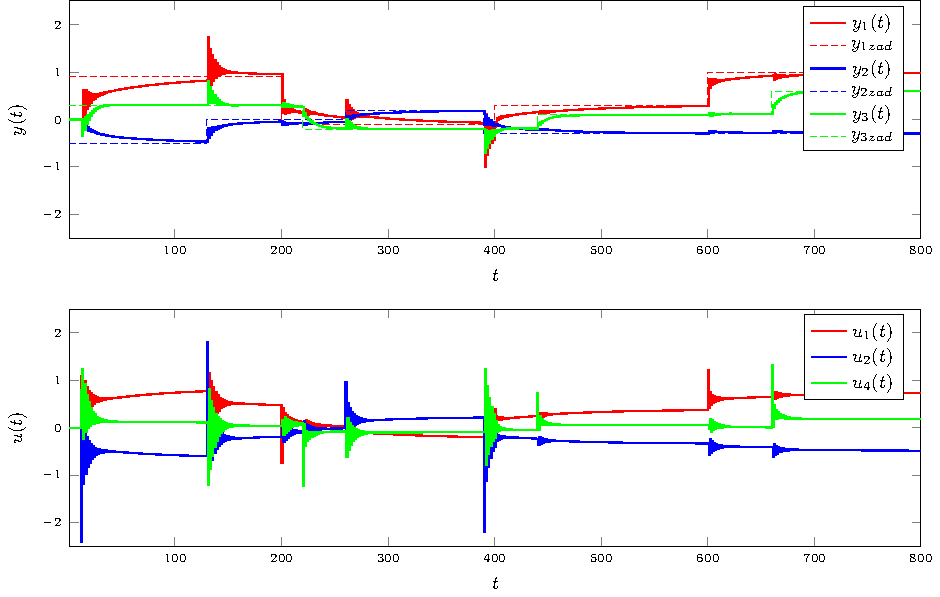
\includegraphics[scale=1]{../wykresy/zad4_pid_1_1.pdf}
	\caption{$Kp = [1, 1.6, 1]; Ti = [20, 20, 15]; Td= [0.1, 1, 0.8]; E = 4.837103e+01$}
\end{figure}

\begin{figure}[H]
	\centering
	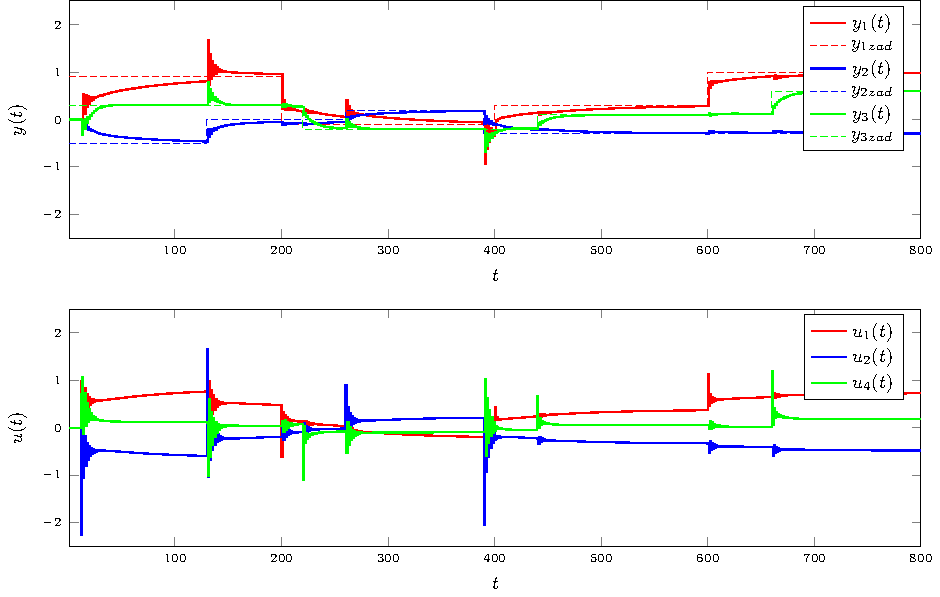
\includegraphics[scale=1]{../wykresy/zad4_pid_1_2.pdf}
	\caption{$Kp = [0.9, 1.5, 0.9]; Ti = [20, 20, 15]; Td= [0.1, 1, 0.8]; E = 5.085968e+01$}
\end{figure}

\begin{figure}[H]
	\centering
	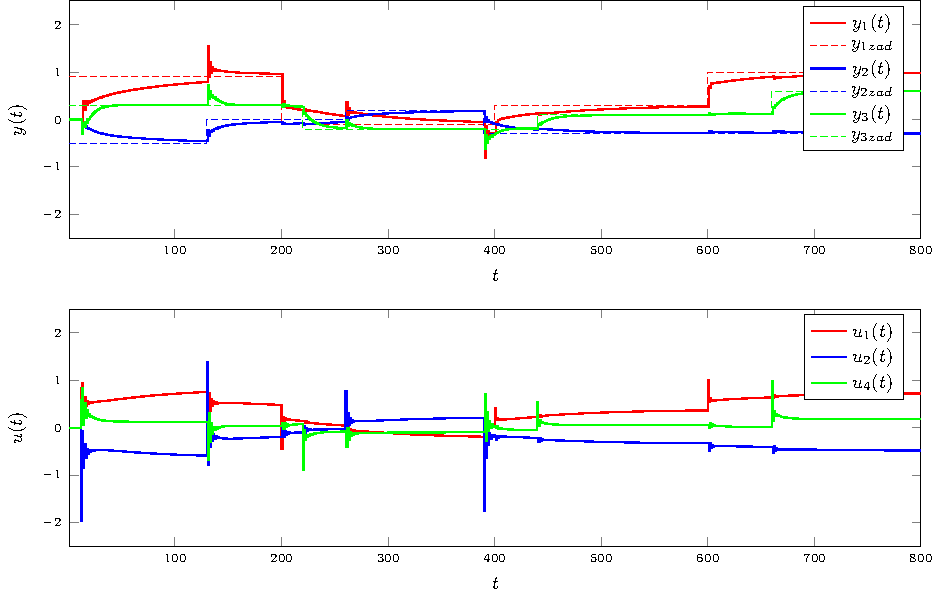
\includegraphics[scale=1]{../wykresy/zad4_pid_1_3.pdf}
	\caption{$Kp = [0.8, 1.4, 0.8]; Ti = [20, 20, 15]; Td= [0.7, 0.9, 0.7]; E = 5.498667e+01$}
\end{figure}


\section*{Konfiguracja $u_1(y_1), u_2(y_3), u_4(y_2)$}
% pid 2

\begin{figure}[H]
	\centering
	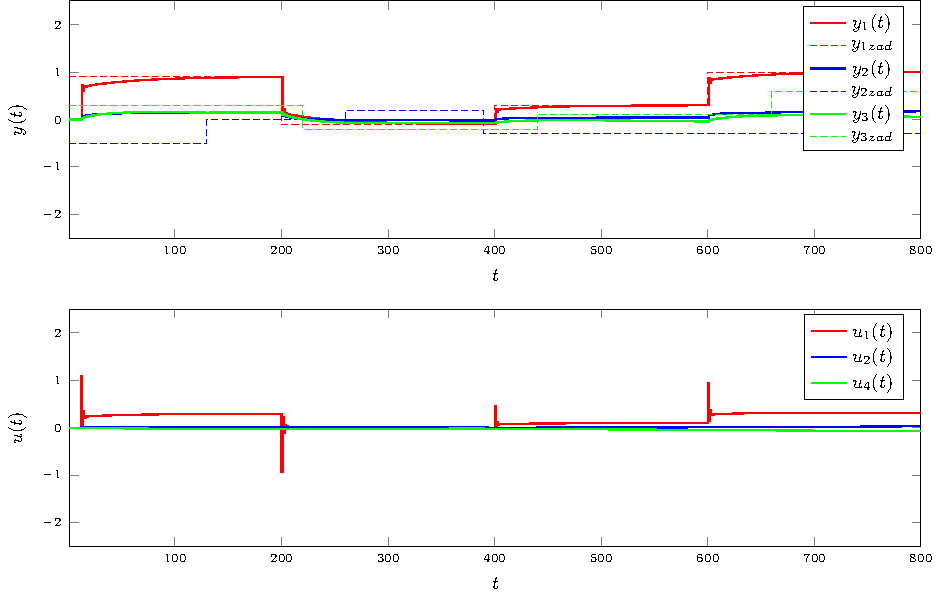
\includegraphics[scale=1]{../wykresy/zad4_pid_2_1.pdf}
	\caption{$Kp = [1, 0.01, 0.01]; Ti = [20, 20, 15]; Ti = [0.1, 0.1, 0.1]; E = 4.837103e+01$}
\end{figure}

\begin{figure}[H]
	\centering
	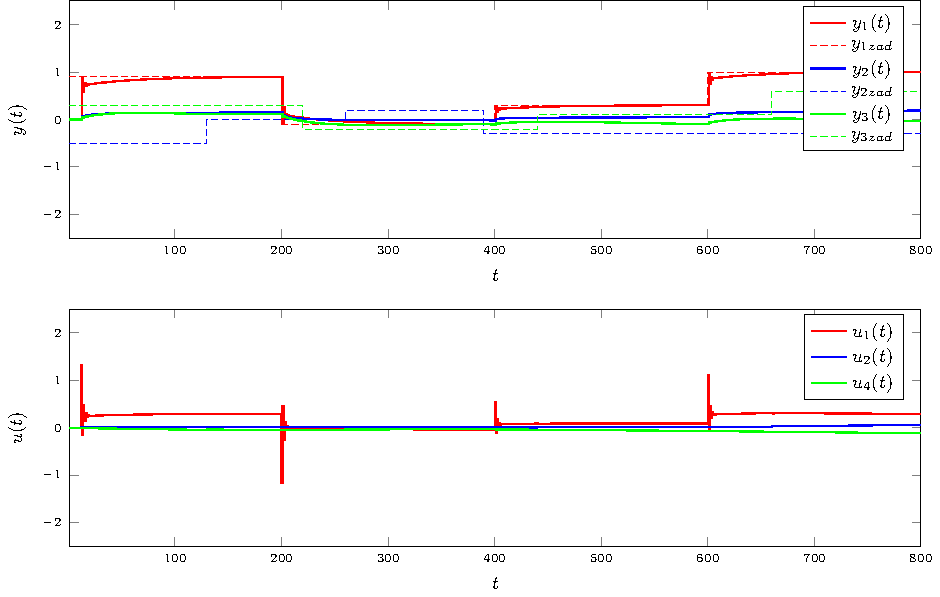
\includegraphics[scale=1]{../wykresy/zad4_pid_2_2.pdf}
	\caption{$Kp = [1.2, 0.015, 0.015]; Ti = [20, 20, 15]; Ti = [0.1, 0.1, 0.1]; E = 1.893750e+02$}
\end{figure}

\begin{figure}[H]
	\centering
	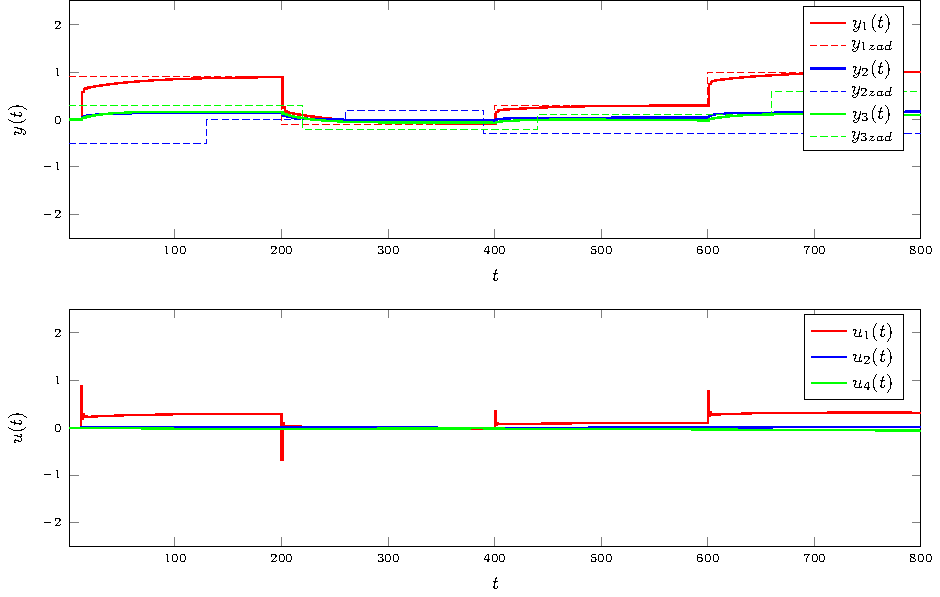
\includegraphics[scale=1]{../wykresy/zad4_pid_2_3.pdf}
	\caption{$Kp = [0.8, 0.008, 0.008]; Ti = [20, 20, 15]; Ti = [0.1, 0.1, 0.1]; E = 5.085968e+01$}
\end{figure}



\section*{Konfiguracja $u_1(y_2), u_2(y_1), u_4(y_3)$}
% pid 3

\begin{figure}[H]
	\centering
	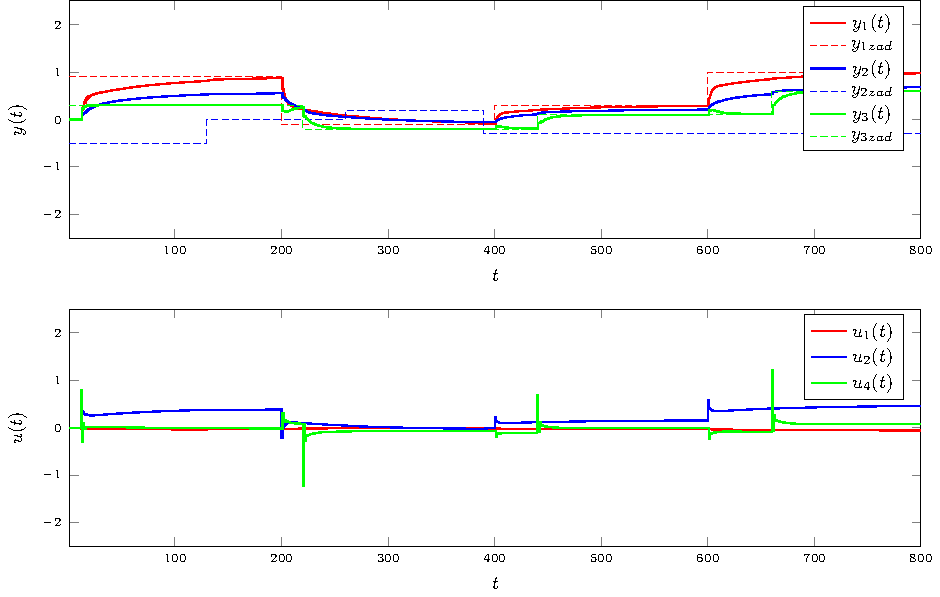
\includegraphics[scale=1]{../wykresy/zad4_pid_3_1.pdf}
	\caption{$Kp = [0.03, 0.5, 1]; Ti = [200, 20, 15]; Ti = [0.01, 0.1, 0.8]; E = 4.837103e+01$}
\end{figure}

\begin{figure}[H]
	\centering
	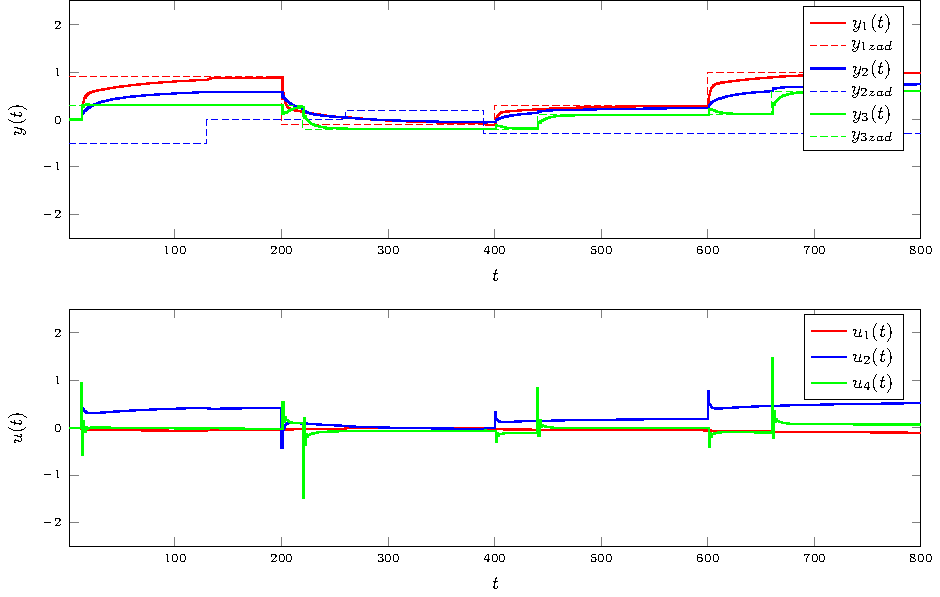
\includegraphics[scale=1]{../wykresy/zad4_pid_3_2.pdf}
	\caption{$Kp = [0.05, 0.7, 1.2]; Ti = [200, 20, 15]; Ti = [0.01, 0.1, 0.8]; E = 1.893750e+02$}
\end{figure}

\begin{figure}[H]
	\centering
	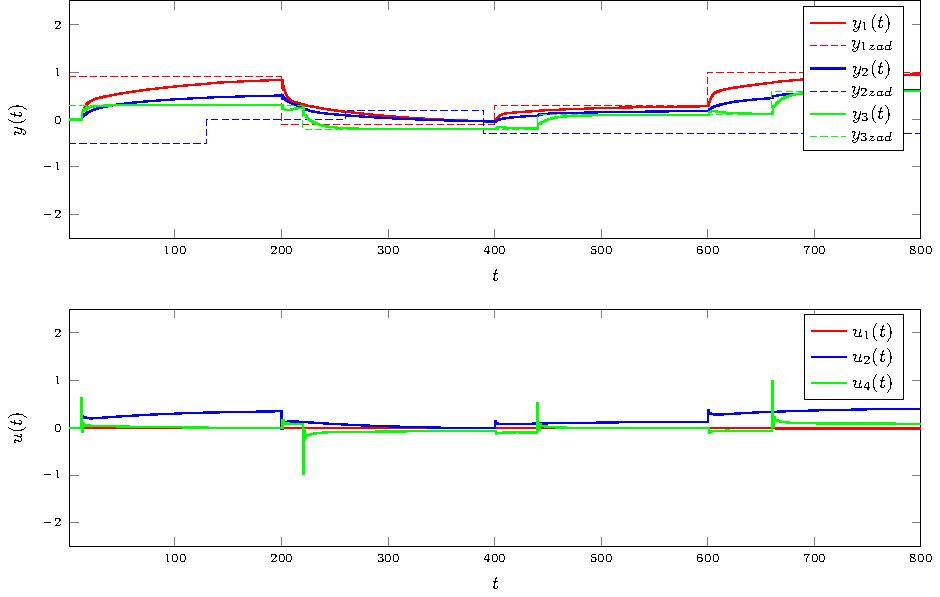
\includegraphics[scale=1]{../wykresy/zad4_pid_3_3.pdf}
	\caption{$Kp = [0.01, 0.3, 0.8]; Ti = [200, 20, 15]; Ti = [0.01, 0.1, 0.8]; E = 3.733132e+02$}
\end{figure}


\section*{Konfiguracja $u_1(y_2), u_2(y_3), u_4(y_1)$}


% pid 4

\begin{figure}[H]
	\centering
	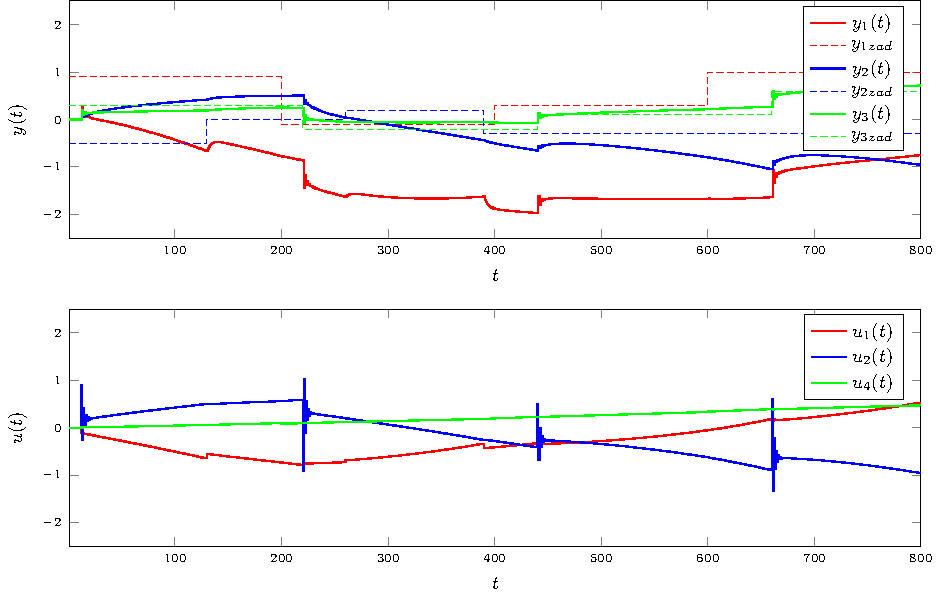
\includegraphics[scale=1]{../wykresy/zad4_pid_4_1.pdf}
	\caption{$Kp = [0.2, 1, 0.01]; Ti = [20, 20, 15]; Ti = [0.01, 1, 0.2]; E = 4.837103e+01$}
\end{figure}

\begin{figure}[H]
	\centering
	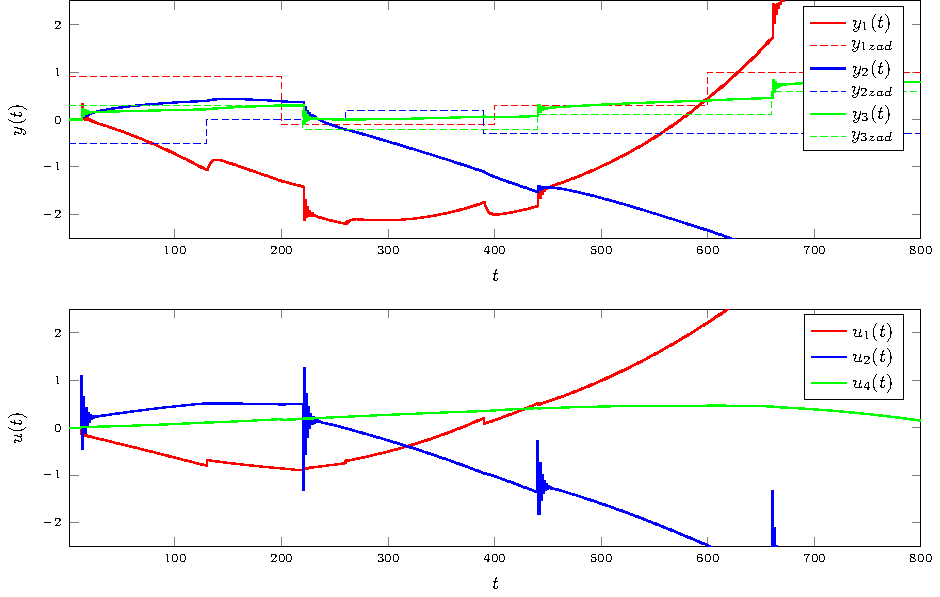
\includegraphics[scale=1]{../wykresy/zad4_pid_4_2.pdf}
	\caption{$Kp = [0.25, 1.2, 0.015]; Ti = [20, 20, 15]; Ti = [0.01, 1, 0.2]; E = 1.893750e+02$}
\end{figure}

\begin{figure}[H]
	\centering
	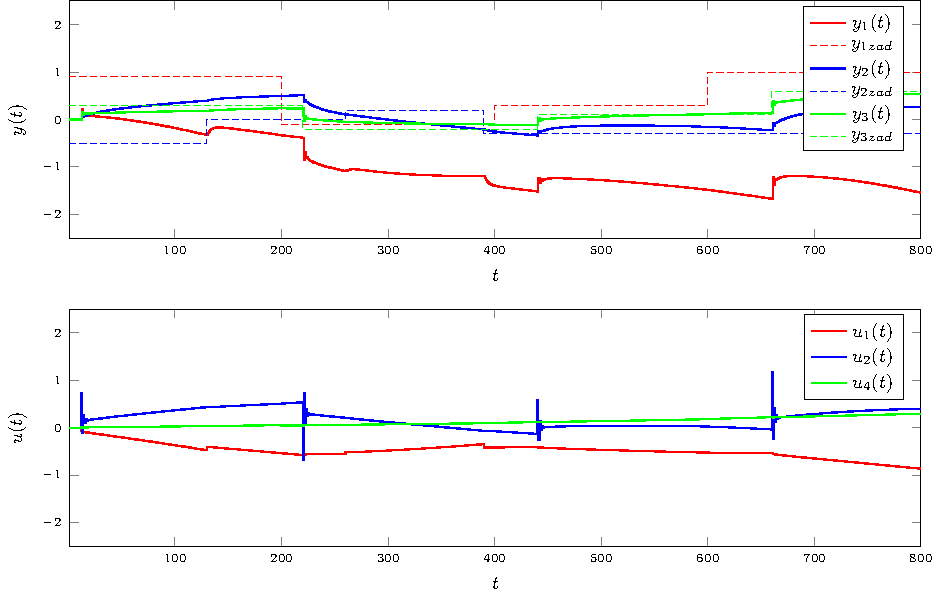
\includegraphics[scale=1]{../wykresy/zad4_pid_4_3.pdf}
	\caption{$Kp = [0.15, 0.8, 0.007]; Ti = [20, 20, 15]; Ti = [0.01, 1, 0.2]; E = 3.733132e+02$}
\end{figure}


\section*{Konfiguracja $u_1(y_3), u_2(y_1), u_4(y_2)$}

% pid 5

\begin{figure}[H]
	\centering
	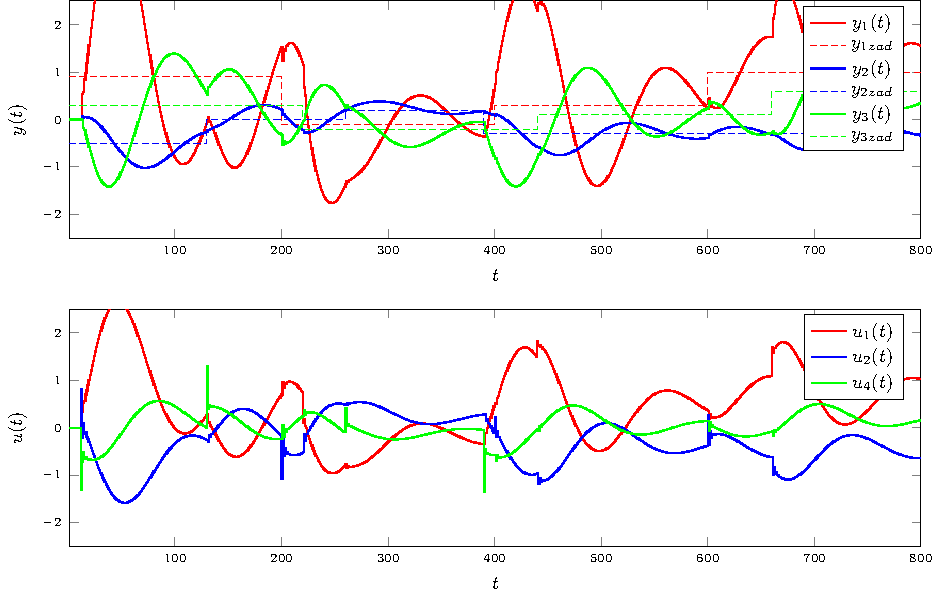
\includegraphics[scale=1]{../wykresy/zad4_pid_5_1.pdf}
	\caption{$Kp = [1, 0.3, 1]; Ti = [20, 20, 15]; Ti = [0.1, 1, 0.8]; E = 4.837103e+01$}
\end{figure}

\begin{figure}[H]
	\centering
	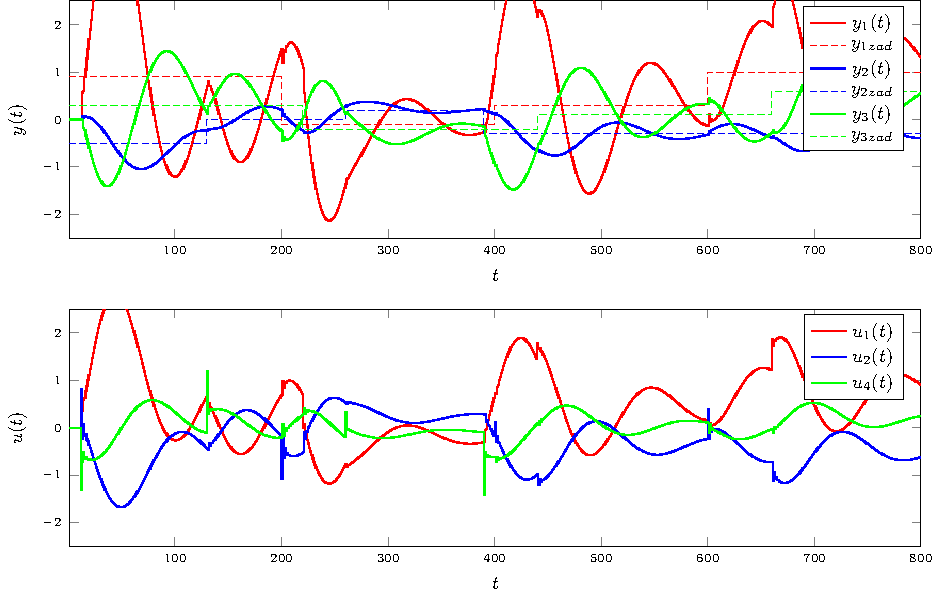
\includegraphics[scale=1]{../wykresy/zad4_pid_5_2.pdf}
	\caption{$Kp = [1.1, 0.3, 1]; Ti = [20, 20, 15]; Ti = [0.1, 1, 0.8]; E = 1.893750e+02$}
\end{figure}

\begin{figure}[H]
	\centering
	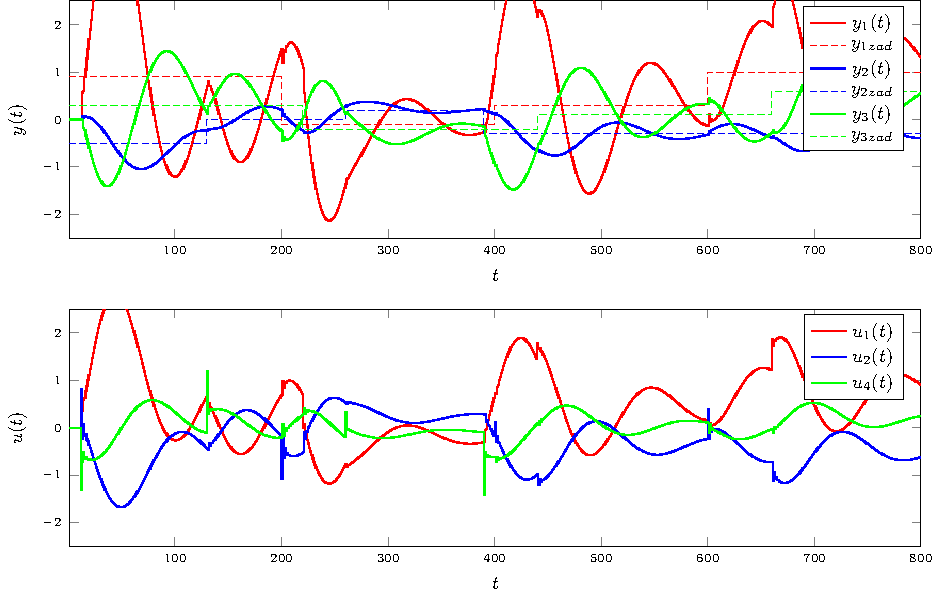
\includegraphics[scale=1]{../wykresy/zad4_pid_5_3.pdf}
	\caption{$Kp = [1.1, 0.3, 1]; Ti = [20, 20, 15]; Ti = [0.1, 1, 0.8]; E = 3.733132e+02$}
\end{figure}


\section*{Konfiguracja $u_1(y_3), u_2(y_2), u_4(y_1)$}

% pid 6

\begin{figure}[H]
	\centering
	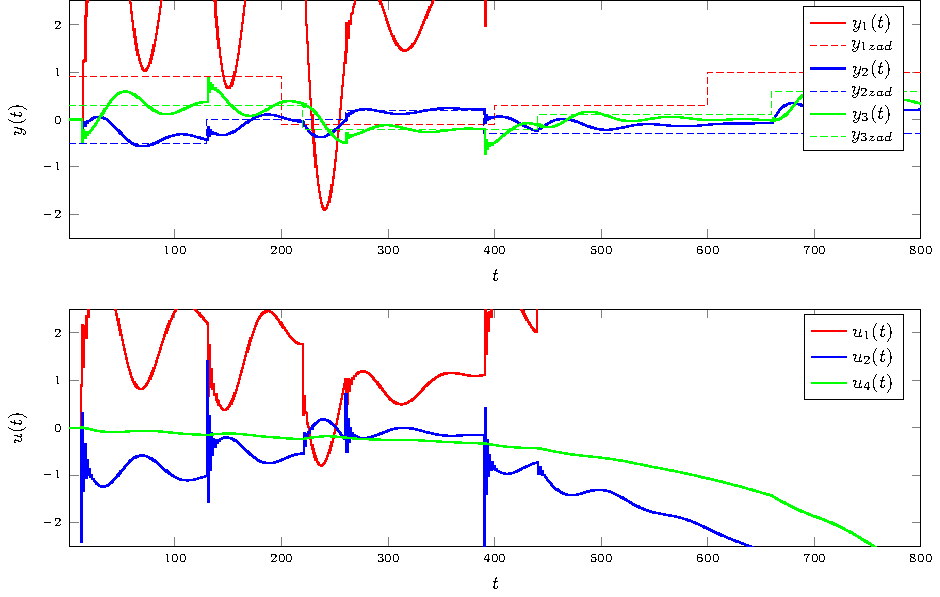
\includegraphics[scale=1]{../wykresy/zad4_pid_6_1.pdf}
	\caption{$Kp = [2, 1.6, 0.01]; Ti = [3, 20, 15]; Ti = [0.2, 1, 0.01]; E = 4.837103e+01$}
\end{figure}

\begin{figure}[H]
	\centering
	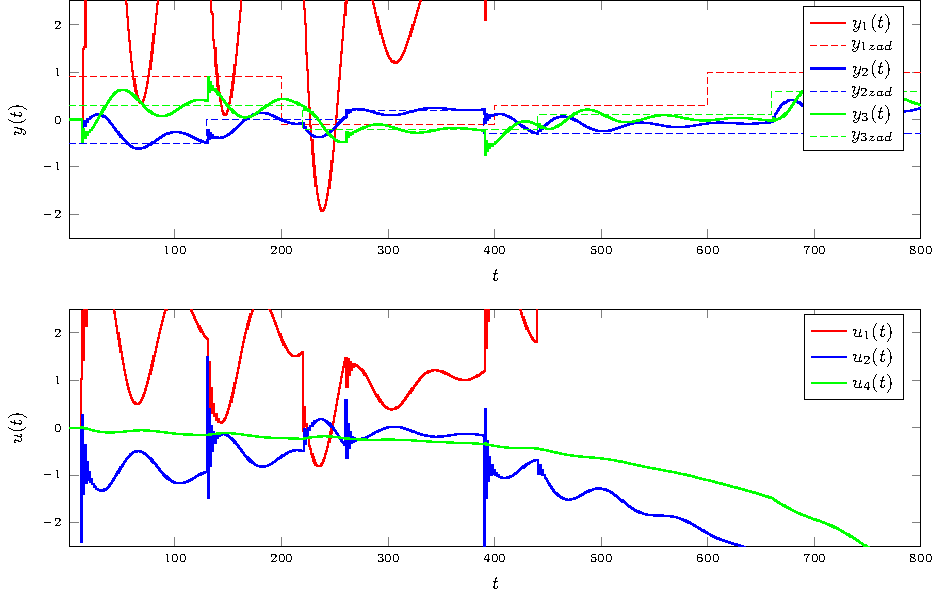
\includegraphics[scale=1]{../wykresy/zad4_pid_6_2.pdf}
	\caption{$Kp = [2.3, 1.6, 0.01]; Ti = [3, 20, 15]; Ti = [0.2, 1, 0.01]; E = 1.893750e+02$}
\end{figure}

\begin{figure}[H]
	\centering
	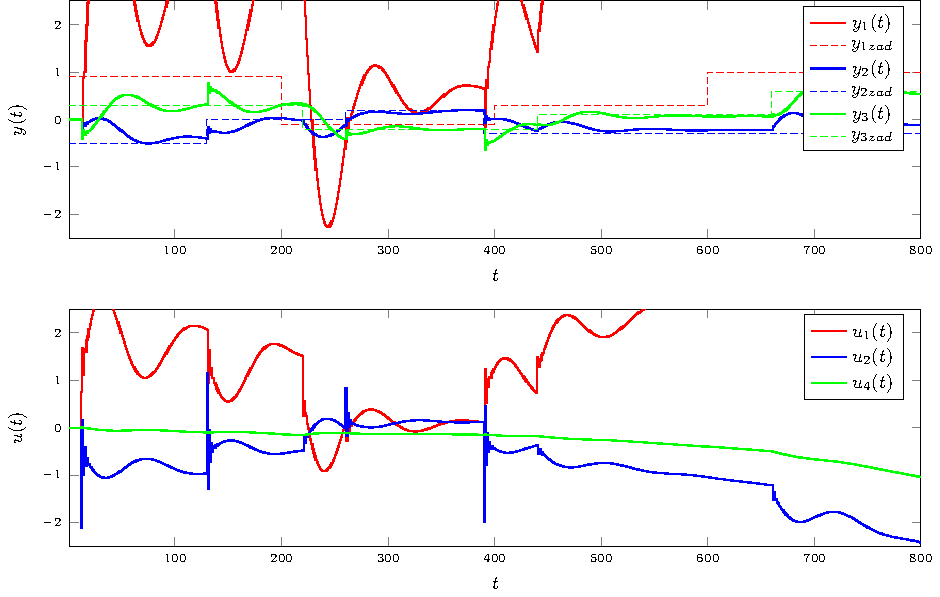
\includegraphics[scale=1]{../wykresy/zad4_pid_6_3.pdf}
	\caption{$Kp = [1.7, 1.4, 0.008]; Ti = [3, 20, 15]; Ti = [0.2, 1, 0.01]; E = 3.733132e+02$}
\end{figure}


\chapter*{Zad. 4 DMC}

Poniżej przedstawione zostały eksperymenty przeprowadzone w celu doboru parametrów regulatora DMC. Przyjęte horyzonty \verb=D, N, Nu= są stałe i równe $200$. Najlepszym regulatorem okazał się ten o parametrach $\lambda$ dla wszystkich wyjść równych 1.


\begin{figure}[H]
	\centering
	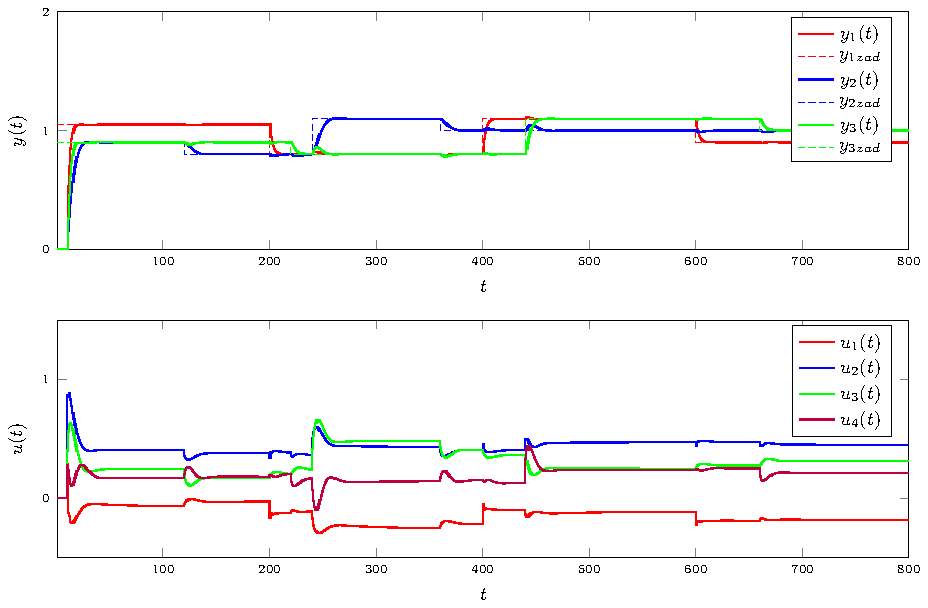
\includegraphics[scale=1]{../wykresy/zad4_dmc_1.pdf}
	\caption{$\lambda = [1, 1, 1, 1]; E = 6.782371e+00$}
\end{figure}


\begin{figure}[H]
	\centering
	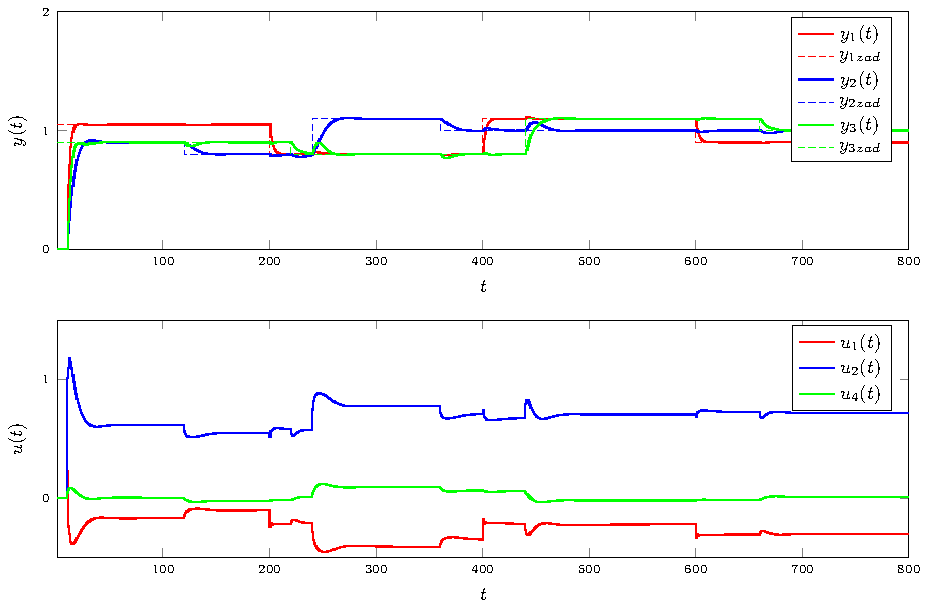
\includegraphics[scale=1]{../wykresy/zad4_dmc_2.pdf}
	\caption{$\lambda = [1, 1, 10, 10]; E = 7.471378e+00$}
\end{figure}


\begin{figure}[H]
	\centering
	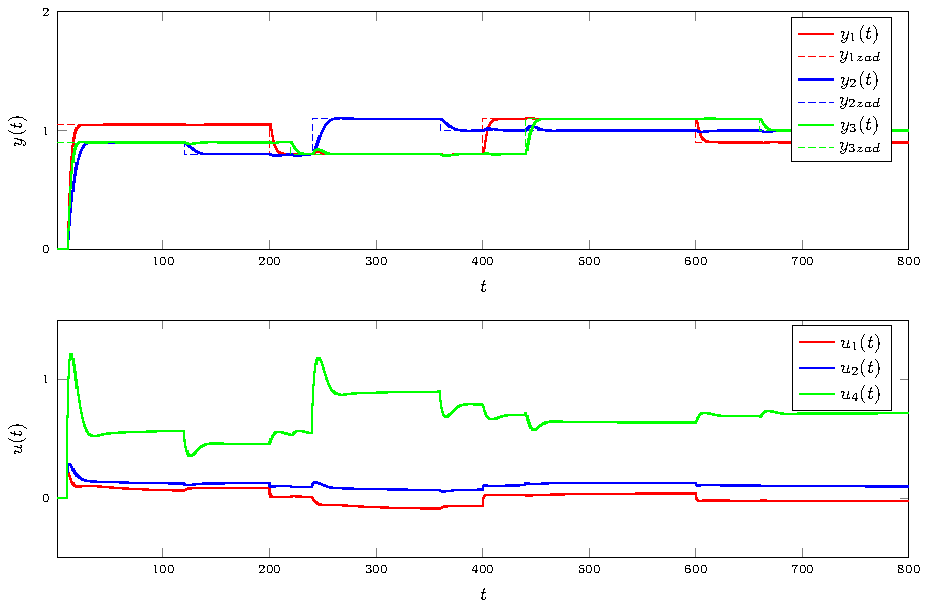
\includegraphics[scale=1]{../wykresy/zad4_dmc_3.pdf}
	\caption{$\lambda = [10, 10, 1, 1]; E = 8.764891e+00$}
\end{figure}


\chapter*{Zad. 5}

Efektem optymalizacji narzędziem \verb=fmincon= były bardzo dobre regulatory PID i DMC.\\\\ Dla regulatora PID dobrane nastawy to: $Kp = [1.476614e+00, 2.671015e+00, 7.194553e+00]; Ti = [7.871889e-01, 5.117763e+00, 2.510283e+01]; Td = [1.452739e-05, 1.339040e-05, 5.285899e-06]$. Błąd dla tych parametrów to $2.014176e+01$ (prawie połowę mniejszy niż dla ręcznie dobieranych nastaw).\\\\ Dla regulatora DMC optymalne parametry to: $\lambda = [3.175234e+06, 2.999843e+05, 8.965576e+05, 1.348709e+06]; \psi = [9.283792e+05, 7.356580e+06, 2.429324e+06]$. Horyzonty, tak samo jak w zadaniu 4, są równe $200$. Błąd regulatora DMC wyniósł $4.856781e+00$ (pięciokrotnie mniejszy niż błąd regulatora PID). Regulator DMC korzysta ze wszystkich wyjść, co daje mu większe możliwości optymalizacji regulacji zględem regulatora PID korzystającego z trzech sygnałów sterujących. Dodatkowo, regulator DMC reguluje wszystkimi wartościami jako całością, w przeciwieństwie do regulatora PID regulującego wartościami osobno (tak naprawdę regulator PID wielowejściowy to kilka regulatorów jednowejściowych).


\begin{figure}[H]
	\centering
	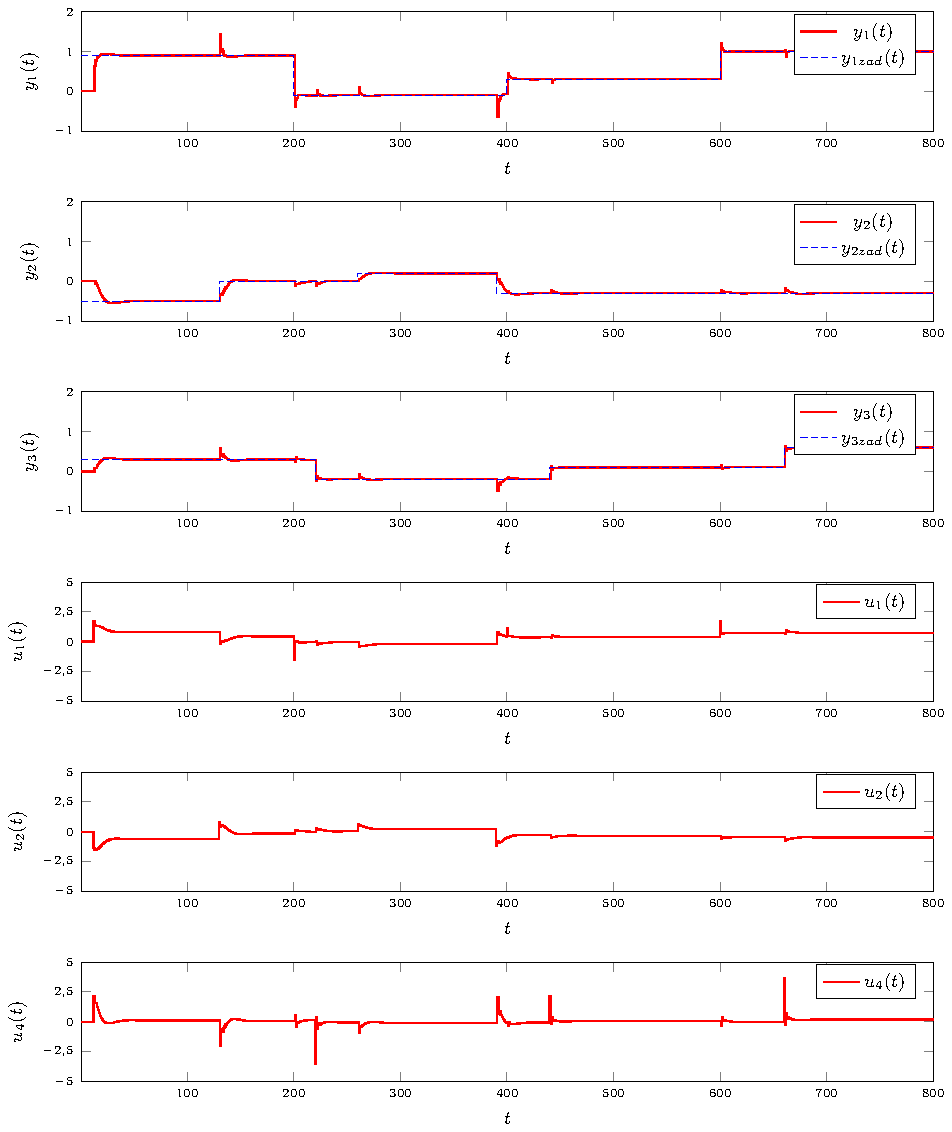
\includegraphics[scale=1]{../wykresy/zad5_pid.pdf}
	\caption{Regulator PID}
\end{figure}

\begin{figure}[H]
	\centering
	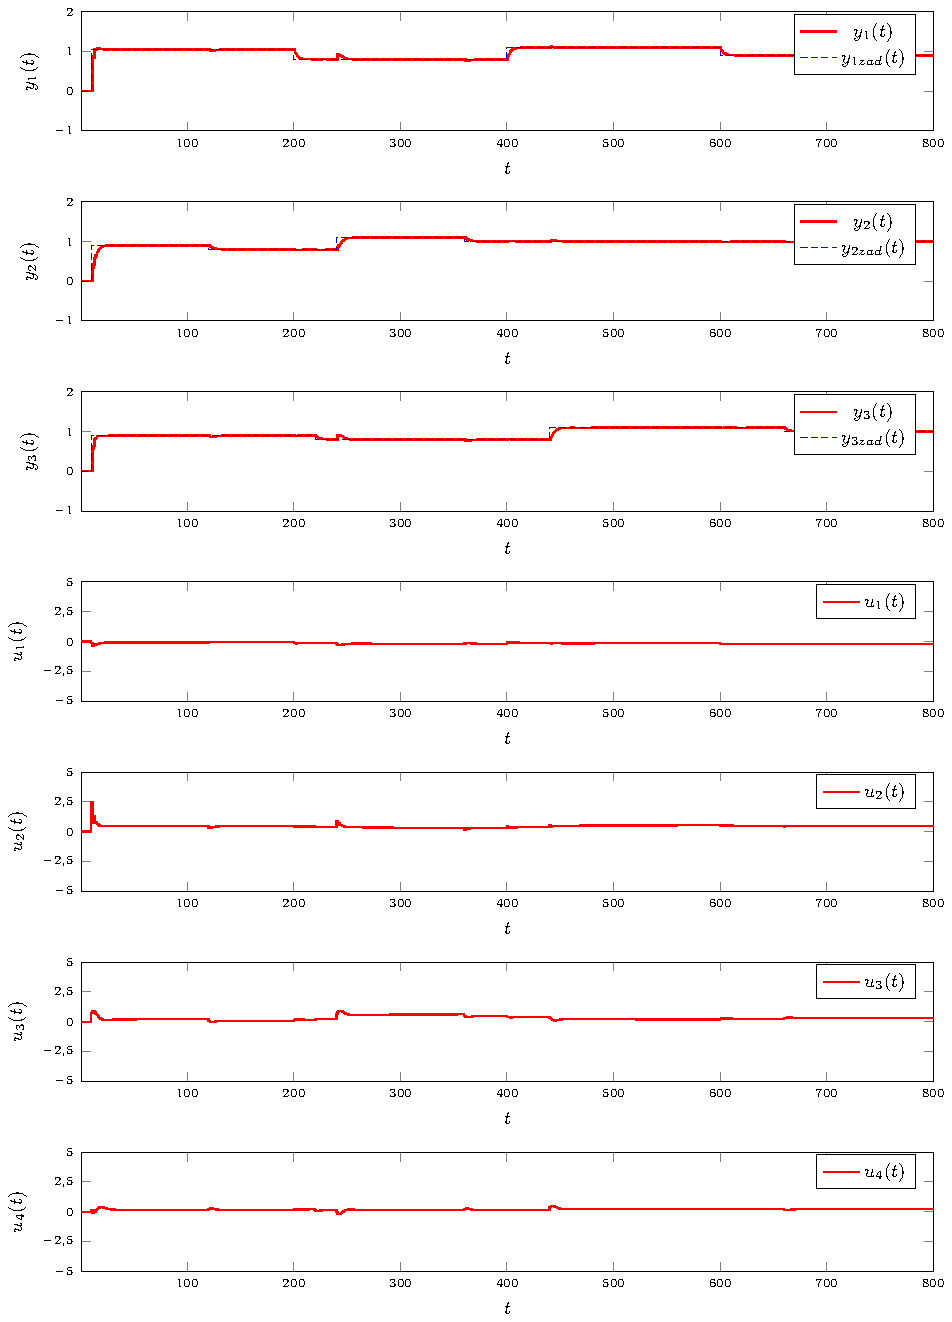
\includegraphics[scale=1]{../wykresy/zad5_dmc.pdf}
	\caption{Regulator DMC}
\end{figure}



\chapter*{Zad. 6}

Został zaimplementowany regulator DMC w wersji możliwie oszczędnej obliczeniowo. Efekt działania regulatora jest identyczny z tym z zadania 4 (eksperymenty przeprowadzone dla tych samych parametrów i wartości zadanych). Poniżej zamieszczone są wykresy z eksperymentów. Nie zostały zamieszczone wykresy porównawcze, ponieważ są one dokładnie identyczne.

\begin{lstlisting}[style=Matlab-editor]

function [ y, u, E, yzad ] = policzDMCZad6(D_, N_, Nu_,
                lambda, psi, Kk_)
N = N_;
Nu = Nu_;
D=D_;

Su1y1 = load('wykresy_pliki/zad2/odp_skok/odpskok_y1_u_1.txt');
Su2y1 = load('wykresy_pliki/zad2/odp_skok/odpskok_y1_u_2.txt');
Su3y1 = load('wykresy_pliki/zad2/odp_skok/odpskok_y1_u_3.txt');
Su4y1 = load('wykresy_pliki/zad2/odp_skok/odpskok_y1_u_4.txt');
Su1y2 = load('wykresy_pliki/zad2/odp_skok/odpskok_y2_u_1.txt');
Su2y2 = load('wykresy_pliki/zad2/odp_skok/odpskok_y2_u_2.txt');
Su3y2 = load('wykresy_pliki/zad2/odp_skok/odpskok_y2_u_3.txt');
Su4y2 = load('wykresy_pliki/zad2/odp_skok/odpskok_y2_u_4.txt');
Su1y3 = load('wykresy_pliki/zad2/odp_skok/odpskok_y3_u_1.txt');
Su2y3 = load('wykresy_pliki/zad2/odp_skok/odpskok_y3_u_2.txt');
Su3y3 = load('wykresy_pliki/zad2/odp_skok/odpskok_y3_u_3.txt');
Su4y3 = load('wykresy_pliki/zad2/odp_skok/odpskok_y3_u_4.txt');

s11=Su1y1(:,2);
s12=Su2y1(:,2);
s13=Su3y1(:,2);
s14=Su4y1(:,2);
s21=Su1y2(:,2);
s22=Su2y2(:,2);
s23=Su3y2(:,2);
s24=Su4y2(:,2);
s31=Su1y3(:,2);
s32=Su2y3(:,2);
s33=Su3y3(:,2);
s34=Su4y3(:,2);

kk=Kk_;

ny=3;
nu=4;
E1=0;
E2=0;
E3=0;

yzads1 = [1.05 0.8 1.1 0.9];
yzads2 = [0.9 0.8 1.1 1];
yzads3 = [0.9 0.8 1.1 1];

index1 = 1;
index2 = 1;
index3 = 1;
y=zeros(ny,kk);
yzad=zeros(ny,kk);
yzad1 = yzads1(index1);
yzad2 = yzads2(index2);
yzad3 = yzads3(index3);
yzad(1,Kk_) = yzad1;
yzad(2,Kk_) = yzad2;
yzad(3,Kk_) = yzad3;
u = zeros(nu, kk);
du = zeros(nu, kk);
dUP = zeros((D-1)*nu, 1);
Y = zeros(N*ny, 1);
Yzad = zeros(N*ny, 1);

M = cell(N,Nu);

for i = 1 : N
   for j = 1 : Nu
      if (i >= j)
         M(i, j)={[s11(i-j+1) s12(i-j+1) s13(i-j+1) s14(i-j+1);...
                  s21(i-j+1) s22(i-j+1) s23(i-j+1) s24(i-j+1);...
                  s31(i-j+1) s32(i-j+1) s33(i-j+1) s34(i-j+1)]};
      else
          M(i, j)={zeros(ny, nu)};
      end
   end
end

M = cell2mat(M);
MP = cell(N, D-1);

for i = 1 : N
   for j = 1 : D-1
      if i + j <= D
         MP(i, j) = {[s11(i+j)-s11(j) s12(i+j)-s12(j) 
			 s13(i+j)-s13(j) s14(i+j)-s14(j);...
            s21(i+j)-s21(j) s22(i+j)-s22(j)
 			 s23(i+j)-s23(j) s24(i+j)-s24(j);...
            s31(i+j)-s31(j) s32(i+j)-s32(j)
			 s33(i+j)-s33(j) s34(i+j)-s34(j)]};
      else
         MP(i, j) = {[s11(D)-s11(j) s12(D)-s12(j)
 			 s13(D)-s13(j) s14(D)-s14(j);...
            s21(D)-s21(j) s22(D)-s22(j)
			 s23(D)-s23(j) s24(D)-s24(j);...
            s31(D)-s31(j) s32(D)-s32(j)
			 s33(D)-s33(j) s34(D)-s34(j)]};
      end
   end
end

MP = cell2mat(MP);

LAMBDA = cell(Nu,Nu);

for i = 1 : Nu
    for j = 1 : Nu
        if i == j
            LAMBDA(i, j)={diag(lambda)};
        else
            LAMBDA(i, j)={zeros(nu, nu)};
        end
    end
end

LAMBDA = cell2mat(LAMBDA);

PSI = cell(N,N);

for i = 1 : N
    for j = 1 : N
        if i == j
            PSI(i, j)={diag(psi)};
        else
            PSI(i, j)={zeros(ny, ny)};
        end
    end
end

PSI = cell2mat(PSI);

K = (M'*PSI*M+LAMBDA)^(-1)*M'*PSI;
K1 = K(1 : nu, :);

ku = K1 * MP;
ke = zeros(4, 3);
ke(1, 1) = sum(K(1, 1 : 3 : (N*ny)));
ke(1, 2) = sum(K(1, 2 : 3 : (N*ny)));
ke(1, 3) = sum(K(1, 3 : 3 : (N*ny)));
ke(2, 1) = sum(K(2, 1 : 3 : (N*ny)));
ke(2, 2) = sum(K(2, 2 : 3 : (N*ny)));
ke(2, 3) = sum(K(2, 3 : 3 : (N*ny)));
ke(3, 1) = sum(K(3, 1 : 3 : (N*ny)));
ke(3, 2) = sum(K(3, 2 : 3 : (N*ny)));
ke(3, 3) = sum(K(3, 3 : 3 : (N*ny)));
ke(4, 1) = sum(K(4, 1 : 3 : (N*ny)));
ke(4, 2) = sum(K(4, 2 : 3 : (N*ny)));
ke(4, 3) = sum(K(4, 3 : 3 : (N*ny)));

for k=10:kk
    
    if mod(k, 200) == 0
        index1 = index1 + 1;
        if index1 > length(yzads1)
            index1 = length(yzads1);
        end
        yzad1 = yzads1(index1);
    end
    yzad(1,k) = yzad1;
    
    if mod(k, 120) == 0
        index2 = index2 + 1;
        if index2 > length(yzads2)
            index2 = length(yzads2);
        end
        yzad2 = yzads2(index2);
    end
    yzad(2,k) = yzad2;
    
    if mod(k, 220) == 0
        index3 = index3 + 1;
        if index3 > length(yzads3)
            index3 = length(yzads3);
        end
        yzad3 = yzads3(index3);
    end
    yzad(3,k) = yzad3;
    
    [y(1, k), y(2, k), y(3, k)] = symulacja_obiektu6( ...
            u(1, k-1), u(1, k-2), u(1, k-3), u(1, k-4), ...
            u(2, k-1), u(2, k-2), u(2, k-3), u(2, k-4), ...
            u(3, k-1), u(3, k-2), u(3, k-3), u(3, k-4), ...
            u(4, k-1), u(4, k-2), u(4, k-3), u(4, k-4), ...
            y(1, k-1), y(1, k-2), y(1, k-3), y(1, k-4), ...
            y(2, k-1), y(2, k-2), y(2, k-3), y(2, k-4), ...
            y(3, k-1), y(3, k-2), y(3, k-3), y(3, k-4));
    
    du(:, k) = ke * (yzad(:, k) - y(:, k)) - ku * dUP;
    
    for i = ((D-1) * nu) : -4 : 8
      dUP(i) = dUP(i-4);
      dUP(i-1) = dUP(i-5);
      dUP(i-2) = dUP(i-6);
      dUP(i-3) = dUP(i-7);
    end
    
    dUP(1:4) = du(:,k);
    u(:, k)=u(:, k-1) + du(:, k);
   
end

for k=1:kk
    E1 = E1 + ((yzad(1,k) - y(1,k))^2);
    E2 = E2 + ((yzad(2,k) - y(2,k))^2);
    E3 = E3 + ((yzad(3,k) - y(3,k))^2);
end

E=E1+E2+E3;

end

\end{lstlisting}


\begin{figure}[H]
	\centering
	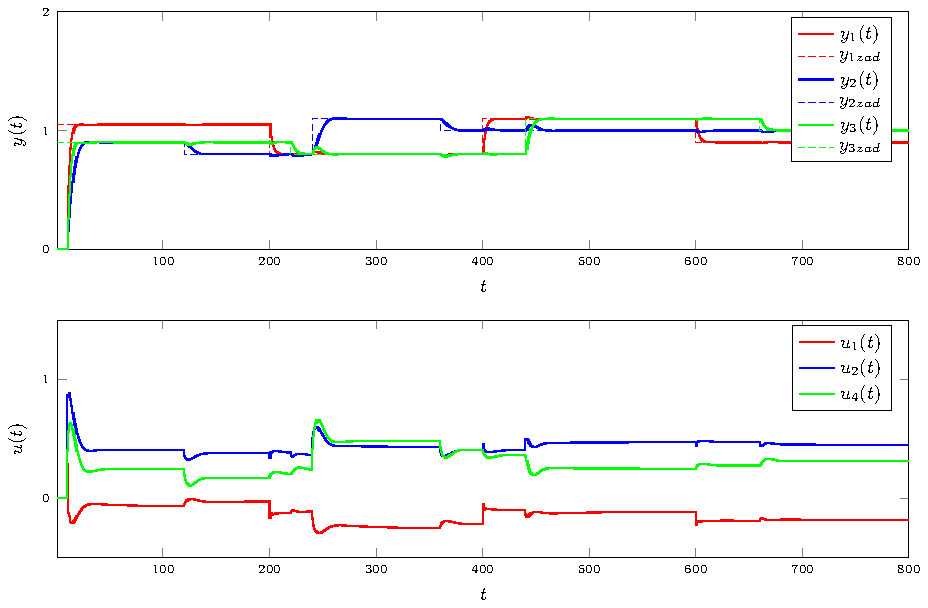
\includegraphics[scale=1]{../wykresy/zad6_dmc_1.pdf}
	\caption{$\lambda = [1, 1, 1, 1]; E = 6.782371e+00$}
\end{figure}


\begin{figure}[H]
	\centering
	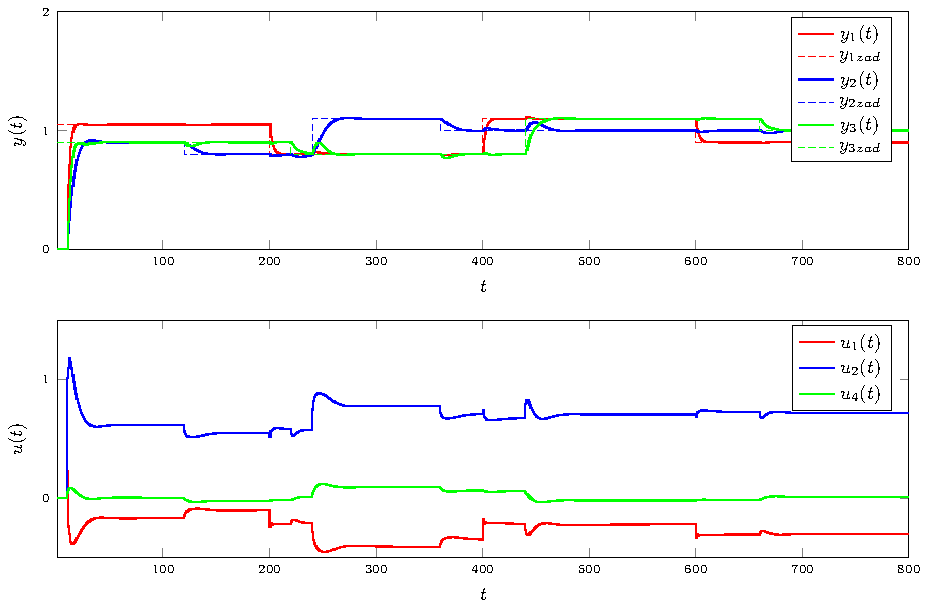
\includegraphics[scale=1]{../wykresy/zad6_dmc_2.pdf}
	\caption{$\lambda = [1, 1, 10, 10]; E = 7.471378e+00$}
\end{figure}


\begin{figure}[H]
	\centering
	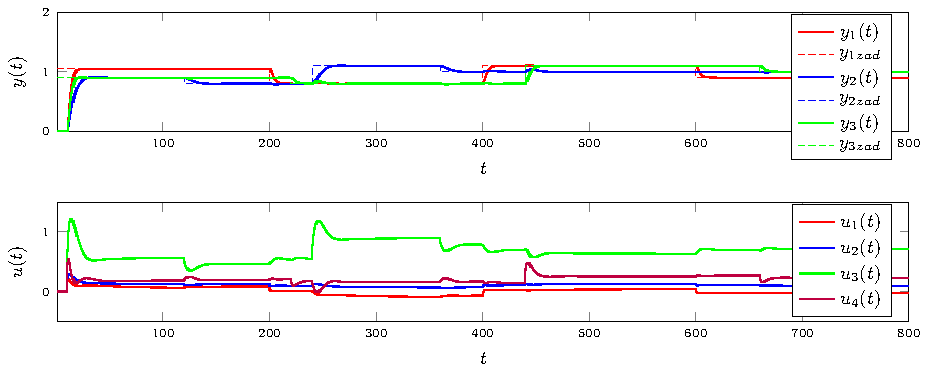
\includegraphics[scale=1]{../wykresy/zad6_dmc_3.pdf}
	\caption{$\lambda = [10, 10, 1, 1]; E = 8.764891e+00$}
\end{figure}



\end{document}


